% !TEX root = main.tex

- The adaptive solar facade was compared with standard facade shading systems and other static BIPV solutions...

\begin{figure}[H]
\begin{center}
\includegraphics[width=10cm, trim= 0cm 0cm 0cm 0cm,clip]{louvres}
\caption{The comparison of the ASF with a static louvered shading system}
\label{fig:louvres}
\end{center}
\end{figure}
% I think I would prefer good old stacked bar plots

\begin{figure}[H]
\begin{center}
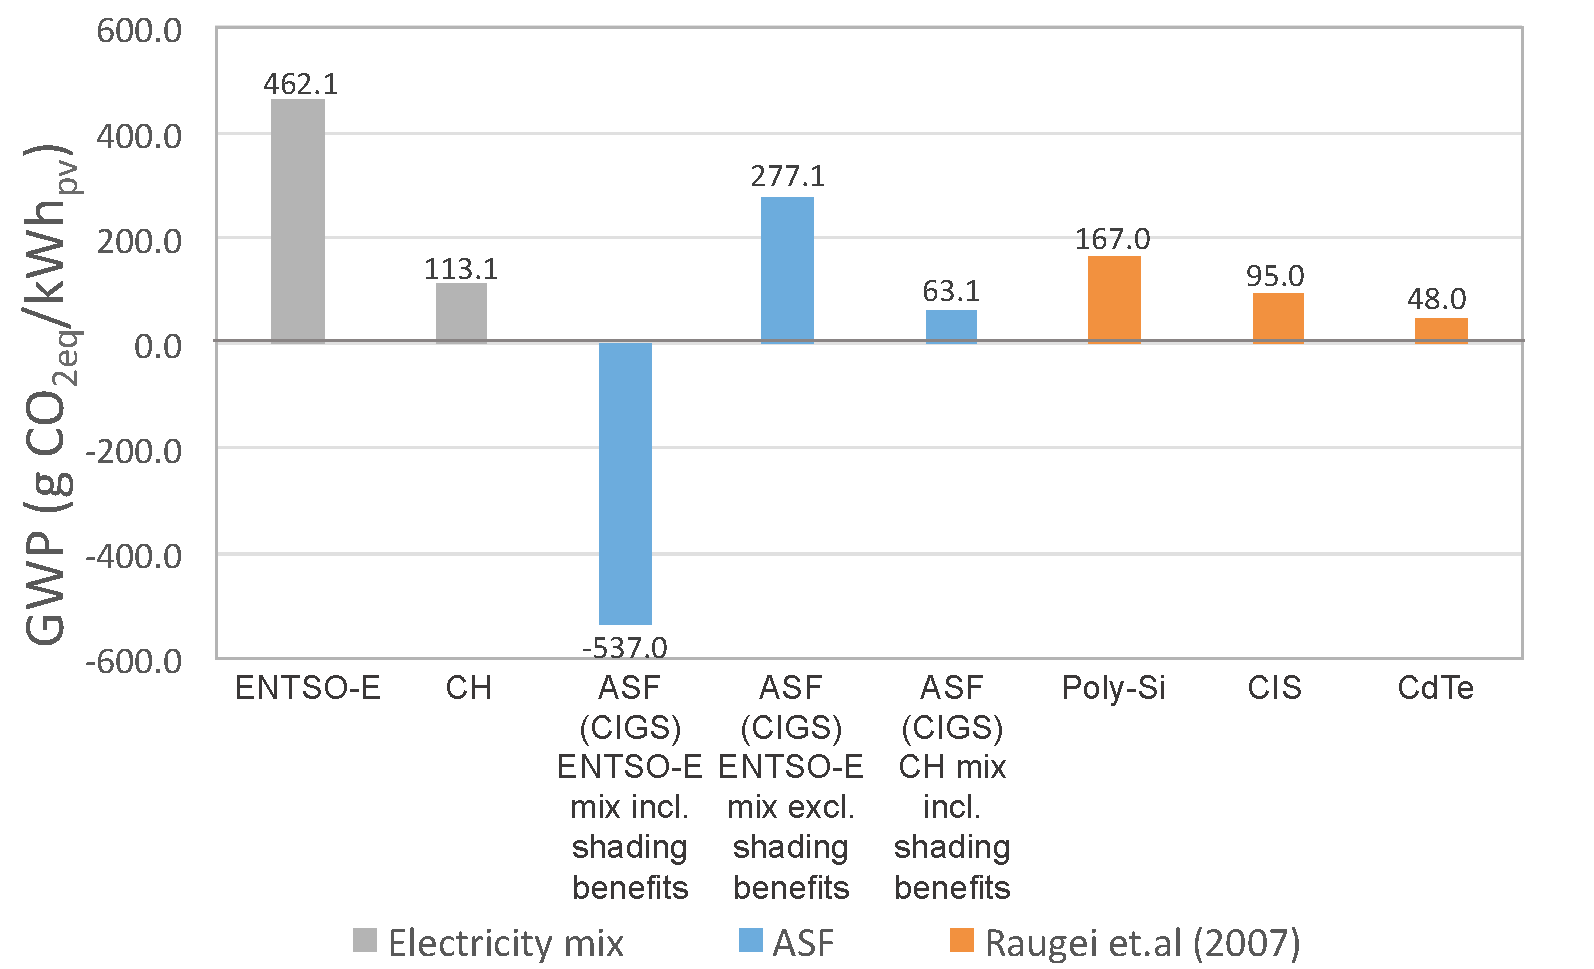
\includegraphics[width=10cm, trim= 0cm 0cm 0cm 0cm,clip]{compPV}
\caption{BIPV comparison of thin-film and BOS}
\label{fig:compPV}
\end{center}
\end{figure}
